\documentclass[11pt, oneside]{article}   	% use "amsart" instead of "article" for AMSLaTeX format
\usepackage{geometry}                		% See geometry.pdf to learn the layout options. There are lots.
\geometry{letterpaper}                   		% ... or a4paper or a5paper or ... 
%\geometry{landscape}                		% Activate for for rotated page geometry
%\usepackage[parfill]{parskip}    		% Activate to begin paragraphs with an empty line rather than an indent
\usepackage{graphicx}				% Use pdf, png, jpg, or eps� with pdflatex; use eps in DVI mode
								% TeX will automatically convert eps --> pdf in pdflatex		
\usepackage{amssymb}
\usepackage{amsmath}

\title{Brief Article}
\author{The Author}
%\date{}							% Activate to display a given date or no date

\begin{document}
\maketitle

\section{Queueing Theory}
This model can be described in a very clean, theoretical way for continuous time; however, to do this, we must disregard the entire graph representing geographical distance. It makes little practical sense to do this for a model that describes behavior in the real world, however, we make a note if because this mathematical theory is well-described.

 Consider a very simplified version of this problem. All taxis wait at a taxi stand and customers arrive to the taxi stand to request a ride. A taxi gives a customer a ride to their destination and returns to the stand with a rate of $\mu$ per timestep $t$. The arrival times of customers are considered random, the waiting time of a customer is called $w$. We want to answer the question of mean waiting time $E[w]$ and the distribution function of $w$, $P(w < c)$.\\

This is a problem in mathematics called queueing theory. We assume exponentially distributed arrival distribution with rate $\lambda$, and $t$ taxis, and infinite customer capacity. This is called a "Multiple Server Model", or $M/M/c/\infty$ model, if we imagine the customers as waiting in a line with multiple taxis are "servers".\\

For this problem, the mean waiting time is given by
\[E[w] = P_0 \frac{\mu \rho^c}{(c -1)! (c \mu - \lambda)^2} \]
And the waiting time distribution is given by
\[ P(w > t) = \frac{P_0 c \rho^c}{c!(c \mu - \lambda)}e^{-(c\mu- \lambda)t} \]
Where $\rho$ is defined by $\lambda/\mu$.

\section{Competing Taxi Companies}
In this model, we consider the case where instead of the three Mythical taxi companies operating through a single dispatcher, three separate companies use separate dispatchers. 

We defined $P_1$, $P_2$, $P_3$ as the percentage of a market that company $1$, $2$, and $3$ control: If the most popular company controls $70\%$ of the market, we assumed a customer will call this company with probability $.7$.\\

\subsection{Naive Model}
Our most naive model is a very simple variation of our model from question $1$.

\begin{itemize}
\item When a customer places a call for a taxi, they call company $i$ with probability $P_i$.
\item The dispatcher for this company radios all the company taxis and gives the job to the taxi who can reach the customer is the shortest time.
\item If all taxis are busy, this time is includes the time for a taxi to finish a job and then pick up the customer.\\
\end{itemize}

Notice that the second two actions are identically the same algorithm from question $1$. In this model, each company chose the minimum number of taxi cabs subject to the earlier constraint that the average customer waiting time be 15 minutes. 


\subsection{Profit Maximization Model}
We then made a couple improvements on this simple models.
\begin{enumerate}
\item When a customer calls a smaller company and is told their wait time is greater than 15 minutes, they call the most popular company and use this taxi service instead.
\item Companies, instead of choosing the minimal number of taxis under the average wait time constraint, choose the best number of taxi cabs by maximizing their expected profit.
\end{enumerate}

\subsubsection{Cost}

\subsubsection{Calculating Profit}
We estimated revenue very simply, as the sum of all taxi fares in trips in a day, where $f_{i,j}$ is the fare for the route from node $i$ to node $j$ and $c_{i,j}$ is a customer calling a taxi to get from node $i$ to node $j$. (We ignore that some companies generate revenue indirectly by renting out taxi cabs to the drivers). The cost matrix $C$ is calculated from the metered price solution in Section 3 above and the distance matrix $A$:  \[C = 1.45A + 2.5 \]

Each company chooses its number of taxicabs T by maximizing the profit equation in a given day, 
\[ \sum_t \sum_{i=1}^{20} \sum_{j=1}^{20} c_{i,j} f_{i,j} - T P  \]

So in this model, while companies do not directly optimize customer waiting times, long waiting times will hurt the revenue as the company loses customers.

\subsection{Results}
We optimized $\text{Pr}_i(t)$, the expected profit for company $i$ with respect to $t$, the total number of cabs by using our result from Section 2 the optimal number of total taxis in Ithaca given the waiting time constraints is $44$. So if $t_i$ is the number of taxicabs owned by Company $i$, we have,
\[t_1 + t_2 +  t_3 = 44\]
So we loop over triangle integer mesh points for $t_1$, $t_2$, $t_3$ to find optimal profits, using the loops below (as $t_3 = 44 - t_1 - t_2$). That is; within this mesh, we calculate expected profit over all possible combinations of $t_1$, $t_2$, $t_3$, given the constraint above.

\begin{verbatim}
 for t1 = 1:3:40
        for t2 = 1:3:43-a

        end
 end
 \end{verbatim}
 
So notice the plot of  $\text{Pr}_1(t)$,  $\text{Pr}_2(t)$, and  $\text{Pr}_3(t)$ has periodic spikes in values: this spike arise naturally as a result of the iterations we used. That is, as the x value of the plot varies from one spike to the beginning of another spike, $t$ for a particular company is being held constant, while all values for the other two companies are being varied. The spikes for the profit plots of Company $2$ and $3$ correspond to the largest Company, Company $1$ having the lowest possible number of taxis. This results in Companies $2$ and $3$ receiving almost all customer calls as Company is quickly overloaded by calls and passengers switch companies as the wait time becomes too high.\\

Analyzing these results, we see that when the taxi companies maximize their profit, we see that the company with a larger share has an optimal number of taxicabs that is larger than the number of taxis in smaller companies. This is the result we expected the model to produce. It is also significant that Company $1$, the much larger company makes much more total net profit (in fact almost twice as much).\\

One can also see that $\text{Pr}_1(t)$, the expected profit for company $1$ with respect to the total number of taxicabs owned by the taxi has a peak at 10 taxicabs and then decreases as the number of cabs continues to decrease. However, $\text{Pr}_2(T)$ and $\text{Pr}_3(t)$, the profit functions for the two smaller companies are decreasing more quickly as the number of cabs the company owns increases.\\

We conclude that the reason for this is that for a company with a small percentage of the market share receives only a small percentage of calls. Therefore after a point, if this company keeps buying taxis, it is not increasing $\sum_t \sum_{i  =1}^20 \sum_{j = 1}^20 c_{i,j} $, the number of calls the company takes in day. However, the cost is increasing linearly in the number of taxis, so the profit goes down.


\begin{figure}[t]
\centering
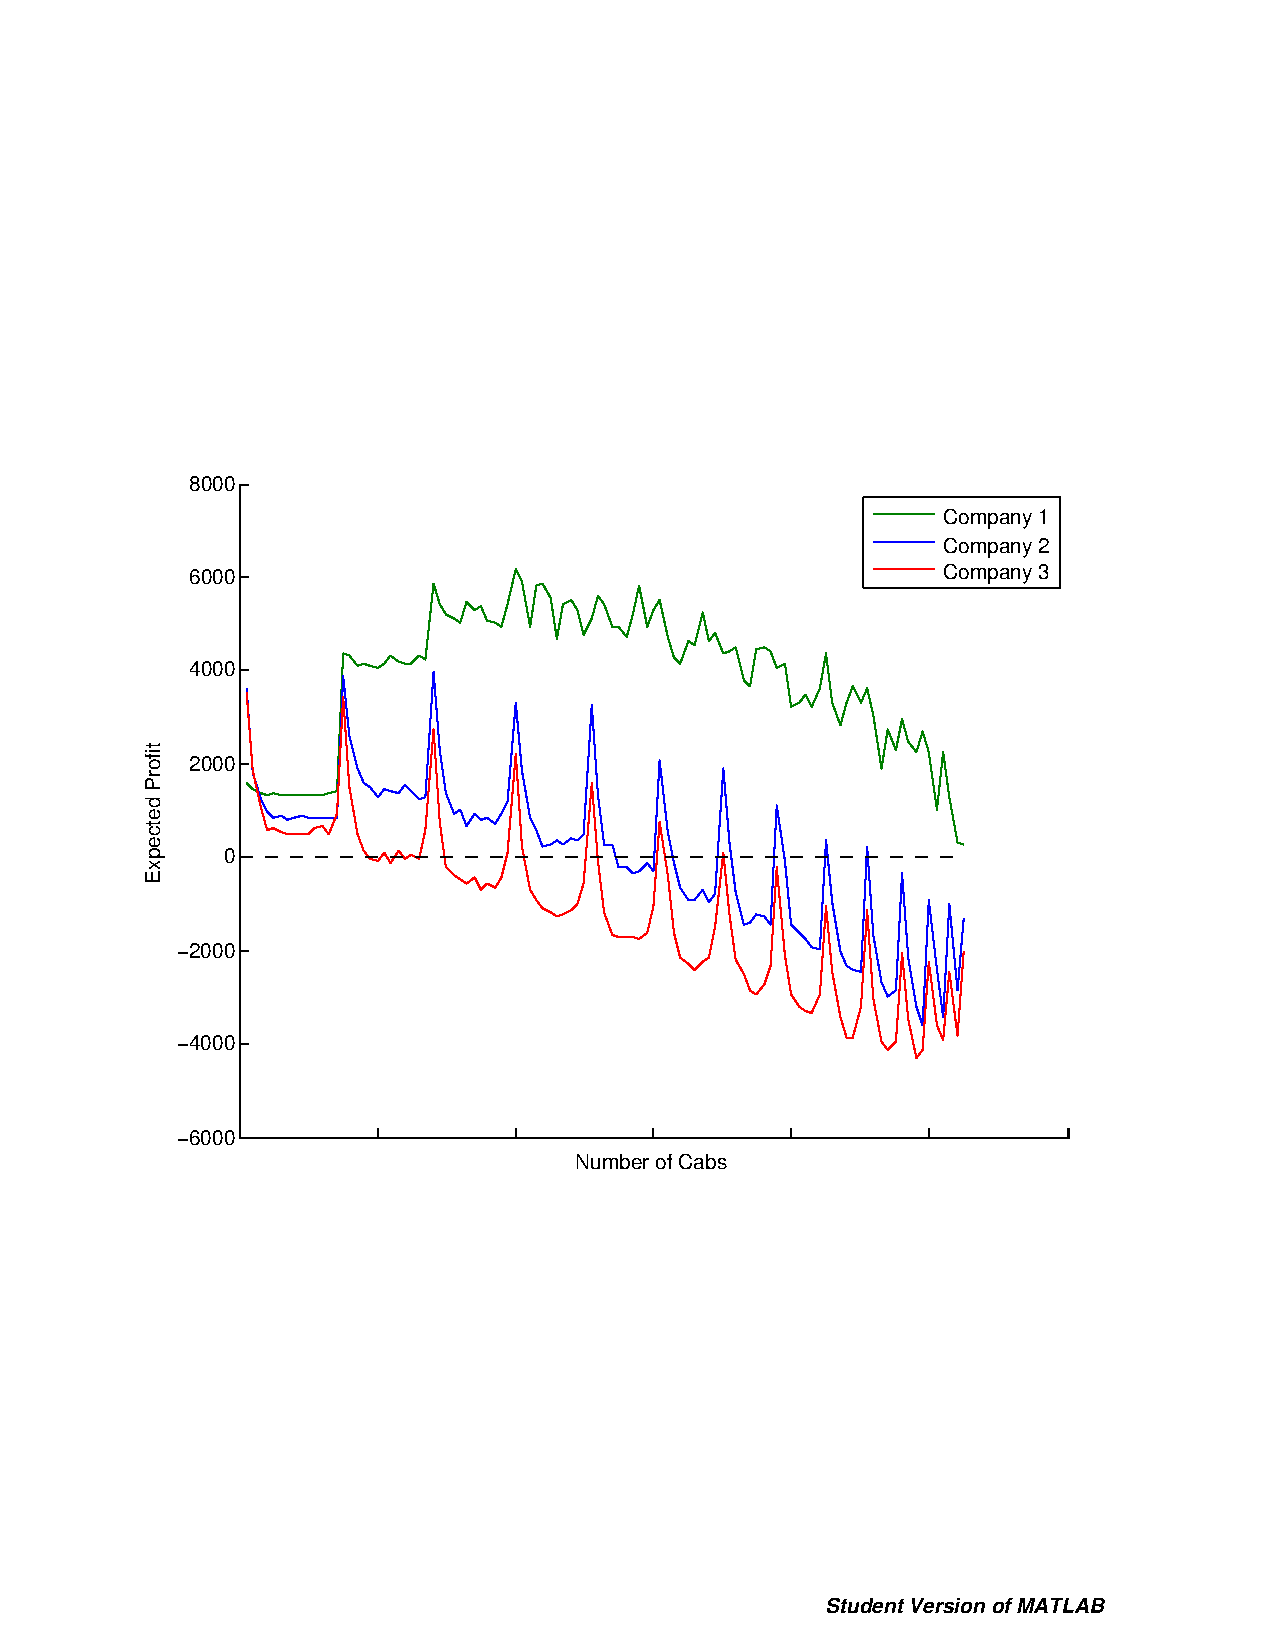
\includegraphics[width=1\textwidth]{prettyplot.pdf}
\caption{}
\label{fig:profits}
\end{figure}

\subsection{Effect of Competition on Average Waiting Time}
Now we compete 

\begin{table}
\centering
\begin{tabular}{ c | c | c  }
Zone \# & $t_i$ maximizing $\text{Pr}_i(t)$ & Average Waiting Time for Company $i$ \\
\hline
Company 1 & 10 cabs &36 minutes\\
Company 2 & 7 cabs& 24 minutes\\
Company 3 & 1 cab & 55 minutes\\
\end{tabular}
\caption{}
\label{tab: prof&wait}
\end{table}




\end{document}  